\section{Experimental comparisons in PEFT}\label{sec:peft-comparisons}

\citet{lee2026learningrate} survey whether vanilla LoRA was evaluated across multiple hyperparameter settings.
We extend this assessment to uncertainty across training runs, validation-based learning-rate selection, disclosure of numerical search spaces and comparable experimental conditions, considering both the proposed method and its principal baseline.

We also review method papers associated with Hugging Face PEFT v0.21.0 \citep{mangrulkar2022peft}, using sources available by September 2026.
The inventory comprises 71 supported entries, 70 identified papers and 64 papers with eligible comparisons between trained methods.
Appendix~\ref{app:peft-review} details the criteria, review procedure and limitations.

Most papers do not clearly establish key experimental controls (\Cref{fig:peft-controls}).
Although shared checkpoints and data are documented in at least one main comparison in 63 and 62 of the 64 papers, respectively, only 25 establish all applicable comparison conditions together, including data exposure, adapted modules and trainable budgets.
Evidence for repeated training and learning-rate selection is even scarcer: only nine document repeated training of both methods with uncertainty attributable to those runs, and seven establish separate validation-based selection from at least three learning rates per method.
Most remaining cases are unclear in the reviewed sources.

\begin{figure}[t]
\centering
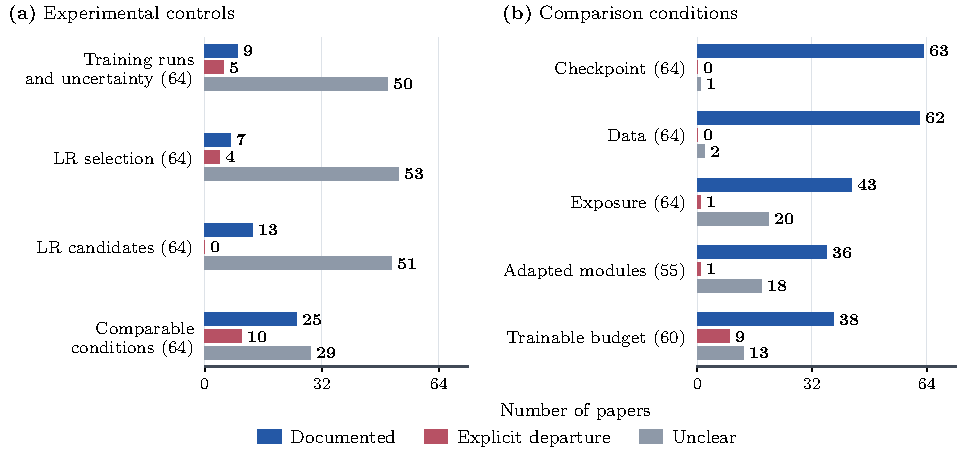
\includegraphics[width=\linewidth]{figures/peft_controls_review.pdf}
\captionsetup{labelsep=period}
\caption{Experimental controls documented in PEFT method papers.
(a) Four controls in the 64 eligible papers.
(b) Components of comparable conditions, excluding inapplicable cases.
Each criterion counts a paper once. Denominators appear in parentheses. Bar lengths and labels show paper counts.
A control is documented when one eligible main comparison meets all applicable requirements.
An explicit departure requires evidence that every eligible comparison fails the definition.
Unclear covers missing or conflicting evidence and unresolved comparison coverage.
Component positives may come from different comparisons.
Definitions and coverage summaries appear in Appendix~\ref{app:peft-review}.}
\label{fig:peft-controls}
\end{figure}

These gaps matter because experimental conditions shape what a comparison can establish.
For example, gains with fewer trainable parameters can support an efficiency claim even when budgets differ.
Comparisons should therefore specify which conditions are comparable, select settings separately for each method and report uncertainty attributable to training runs.

For modest adaptation datasets, independent supervised PEFT runs can be much cheaper than pretraining or rollout-intensive post-training such as reinforcement learning with verifiable rewards (RLVR).
Method-specific learning-rate selection over an exponentially spaced grid and replication across training seeds should therefore be standard practice, with costs that are often manageable.
In RL, higher training costs often limit replication, but DataFlex-RL illustrates why stronger controls matter: its primary comparison of 13 configurations over 12 matched seeds under a common training recipe finds no statistically reliable gains from the tested data policies over their respective baselines \citep{liang2026dataflexrlevaluationplatformrlvr}.
These findings strengthen the case for controlled comparisons in PEFT, where replication is more affordable.
Accordingly, our study combines common experimental settings, method-specific tuning and multiple training seeds to examine task performance and retention.
